
Lentoasentojen opettelu on helppo aloittaa oppilassuorituksista saaduista perusteista. Ennen A-lisenssin saamista olet jo harjoitellut liukua ja sittisasentoa. Tässä luvussa kerrotaan syvällisemmin näistä lentoasennoista sekä hetukka- ja kulmalentämisestä. 

\section{ Kulma }
\label{freefly-lentoasennot-kulma}


Liukuminen on kaikkien hyppääjien tuntema ja käyttämä tekniikka, mutta se on myös freeflyn alalaji, jolloin sitä kutsutaan kulmahyppäämiseksi (Angle, Atmonauti, Tracing, tracking). Hyvä liukuasento mahdollistaa nopean vaakavauhdin ilman että putoamisvauhti kasvaa. Freefly-liukuhyppyjen tarkoituksena ei kuitenkaan ole päästä mahdollisimman kauas muista hyppääjistä, vaan liukua suunnitellussa muodostelmassa. Samassa liukumuodostelmassa voi olla sekä selällään että mahallaan liukujia. Liukuhypyllä voidaan ottaa myös otteita. 


Kulmalentämisellä on useita eri nimityksiä ja osa-alueita. Flokkaaminen on lähes hetukan kaltaista melko pystysuoraan tapahtuvaa lentämistä ja atmonauti on flokkaamisen ja liukumisen välialuetta. Kulmalentämisessä saadaan enemmän vapaapudotusaikaa kuin tavallisessa freefly -hyppäämisessä. Kulmalentohypyn reitin suunnitteluun pätevät samat perusasiat kuin liukuhypynkin. Uloshyppyvuoro pokassa voi olla mikä vain, sillä kulmalentoryhmä liukuu yleensä poispäin hyppylinjasta. Kulmaa voidaan lentää pää edellä mahallaan, pää edellä selällään, jalat edellä mahallaan, jalat edellä selällään tai kyljellään. Kulmalentäminen hallitusti on aluksi vaikeaa. 

\subsection{ Maha maata kohti }
\label{freefly-lentoasennot-maha-maata-kohti}


Hyvään kulma-asentoon pääset seuraavasti: 

\begin{itemize}
\item  ota kiintopiste edestä tai liukuhyppyä johtavasta hyppääjästä 
\item  paina leukaa kiinni rintaan ja olkapäitä eteen saadaksesi aikaan kupin ylävartaloon 
\item  suorista tai jopa koukista lantio – älä taivuta 
\item  pidä käsivarret vartalon vieressä 
\item  jalkojen asentoa säätelemällä säädellään eteenpäin suuntautuvaa nopeutta. 
\end{itemize}

Kulma-asennossa on tärkeää säilyttää vartalon jännitys, jotta liike pysyy stabiilina eikä nyöki. Alussa asentoa on helpoin ohjata käsivarsilla ja kämmenillä. Kun taitosi kasvavat, ohjailu sujuu tehokkaimmin muuttamalla vartalon asentoa hartialinjasta jalkoihin. 


\begin{Figure}\centering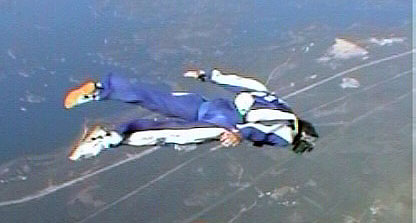
\includegraphics[width=0.95\textwidth]{Liukuasento.jpeg}\captionof{figure}{Liukuasento}\end{Figure} 


Jokaiselle hyppääjälle sopivin liukuasento löytyy kokeilemalla. Asento vaihtelee muun muassa ruumiinrakenteesta johtuen. Myös tavat säädellä vauhtia ja korkeutta eli kulman jyrkkyyttä vaihtelevat, mutta seuraavassa on muutamia vinkkejä, joita voit kokeilla. 

\begin{itemize}
\item  Jos haluat päästä alaspäin eli jyrkemmin, paina otsaa ilmavirtaa vasten ja ylävartaloa alaspäin muuhun vartaloon nähden. Varo kuitenkin, ettet päädy head-down asentoon.  
\item  Ylöspäin eli hitaammin pääset levittämällä liukuasentoa sekä muodostamalla kupin lantiosta. Huomaa, että korkeutta säädellessäsi on tärkeää säilyttää eteenpäin vievä liukuasento. 
\item  Eteenpäin menevää liukunopeutta voit säädellä levittämällä ja kaventamalla asentoasi.  
\item  Jos haluat jarruttaa vaakavauhtia, levitä käsivarret sivuille ja pudota polvia. Vaakavauhtia lisäät kaventamalla asentoasi ja keskittymällä purevaan liukuasentoon. 
\end{itemize}
\subsection{ Selkä maata kohti }
\label{freefly-lentoasennot-selka-maata-kohti}


Selkäliuku vaatii hyvää vartalonhallinta ja vaatii myös taitoa lentää suoraan näkemättä kiintopistettä maasta. Selkäliu´ussa: 

\begin{itemize}
\item  pään tulee olla suorassa linjassa vartalon kanssa niin, ettei se taivu liikaa taakse ja käännä sinua hetukka-asentoon 
\item  keskivartalo muodostaa loivan kaaren, jossa lantio on ylimpänä (purista pakaroita) 
\item  jalat ojennetaan ja niitä painetaan ilmavirtaa vasten 
\item  jalat pidetään lähestulkoon yhdessä, nilkat ojennettuina 
\item  käsivarret ovat hartioiden alapuolella 
\end{itemize}

Tehoton selkäliukuasento hidastaa vaakavauhtia ja nopeuttaa putoamisvauhtia. Yleinen ongelma on se, että selällään liukuja yrittää katsoa perässä tulevia, jolloin pää nousee ylemmäs ja lantio tipahtaa alemmas. 


\begin{Figure}\centering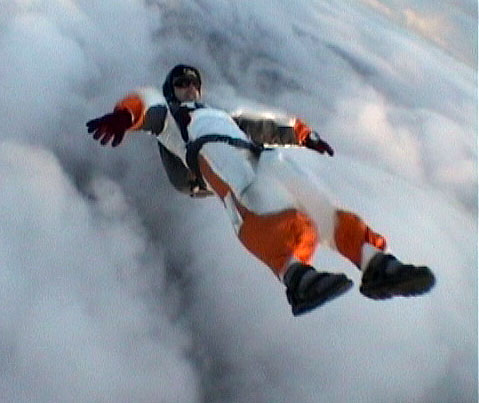
\includegraphics[width=0.9\textwidth]{Liukuasento-selallaan.jpeg}\captionof{figure}{Liuku selällään}\end{Figure} 

\section{ Head-up / Sittis (sitfly) }
\label{freefly-lentoasennot-head-up-sittis-sitfly}


Freefly-hyppäämisen harjoittelu tulee aloittaa sittiksestä. Vasta kun pysyt ongelmitta sittiksessä ja osaat liikkua siinä, voit siirtyä hetukkalentämisen harjoitteluun. Sittis on lentoasento, jossa putoamisvauhti on vastaava kuin hetukkaa lennettäessä, mutta asento on helpompi hallita eikä siinä tapahdu niin paljon tahatonta liikkumista kuin päällään lennettäessä. 

\subsection{ Sittikseen pääseminen }
\label{freefly-lentoasennot-sittikseen-paaseminen}


Uloshyppy suoraan sittikseen tapahtuu helpoiten selkä ilmavirtaan eli selkä koneen menosuuntaan. Pudottaudu ovelta ilmavirtaan, levitä käsivarret ja jalat mahdollisimman yhtäaikaisesti ja yritä pitää asento symmetrisenä. Muista pitää lantio ja jalat vahvoina niin, ettei potkurivirta riko asentoa. Rentoudu, mutta pidä mielessä, mistä ilmavirta tulee äläkä anna sen kaataa sinua. 


Vapaapudotuksessa pääset sittisasentoon selkälennosta tai palloasennosta painamalla jalkapohjat ilmavirtaa vasten, levittäen kädet symmetrisesti sivuille ja nostaen asennon istuvaksi. Pidä katse horisontissa. Mahaltaan boxista voit nousta sittikseen vetämällä polvet rintaan, levittäen kädet symmetrisesti sivuille ja nojaamalla taaksepäin. Paina jalkapohjia ilmavirtaa vasten ja nosta asento istuvaksi. 

\subsection{ Sittiksen perusasento }
\label{freefly-lentoasennot-sittiksen-perusasento}


Sittiksen perusasennossa ylävartalosi on pystysuorassa ja katseesi horisontissa. Kädet ovat sivulla hartialinjan tasalla. Ne voivat olla joko suorina vartalosi sivulla tai ne voivat olla kyynärpäistä taivutetut, jolloin kämmenet ovat hartialinjan etupuolella. Jalat ovat siten, että nilkat, polvet ja lantio muodostavat 90 asteen kulmia taitekohtiinsa. Polvien välinen etäisyys toisiinsa on ainakin hartioiden levyinen, jotta rintakehä ja lantio ovat vapaasti käytettävissä liikkumiseen. Jalat ovat polvien kohdalta 90 asteen kulmassa, eli sääret ovat poissa reisien alta ja jalkapohjat ovat ilmavirtaa vasten. Tässä asennossa putoat paikallaan. 


\begin{Figure}\centering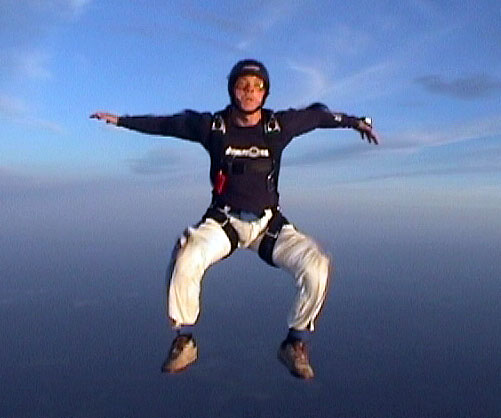
\includegraphics[width=0.95\textwidth]{Sittis.jpeg}\captionof{figure}{Sittisasento}\end{Figure} 


Voit harjoitella sittisasentoa istumalla tuolilla hajareisin. Pidä selkä suorana ja käsivarret sivuille ojennettuina. Tarkista 90 asteen kulmat. Kun katsot suoraan eteenpäin, sinun tulee nähdä kädet näkökentässäsi. Tuolilla istuessa saat kuvan siitä, miltä sittiksen tulisi näyttää. Jotta saat kuvan myös siitä, miltä se tuntuu, laita selkä seinää vasten ja jalkasi sen verran kauemmaksi seinästä, että joudut hieman nojaamaan selälläsi seinään. Pidä leveä haara-asento, vähintäänkin olkapäiden levyinen. Laskeudu selkä seinää vasten nojaten melkein istuvaan asentoon. Hypyn aikana sinun tulee tuntea ilmavirta jalkapohjissasi samaan tapaan kuin tunnet oman painosi jalkapohjissa seinää vasten istuessasi. 

\subsection{ Liikkuminen  eteen-ja taaksepäin sittiksessä }
\label{freefly-lentoasennot-liikkuminen-eteen-ja-taaksepain-sittiksessa}


Sittiksessä liikkuminen tapahtuu lantion avulla. Kun työnnät lantiota eteenpäin, liikut eteenpäin. Eteenpäin liikkumista voit tehostaa kääntämällä kädet hartialinjan taakse kämmenet vasten ilmavirtaa sekä samalla suoristaen hivenen jalkoja. Tämä asento vie sinua tehokkaasti eteenpäin, ja sen hallittu pysäyttäminen vaatii vastaliikkeen. Asento on myös hyvin epävakaa, joten harjoittele sitä aluksi hyvällä etäisyydellä muista hyppääjistä. 


\begin{Figure}\centering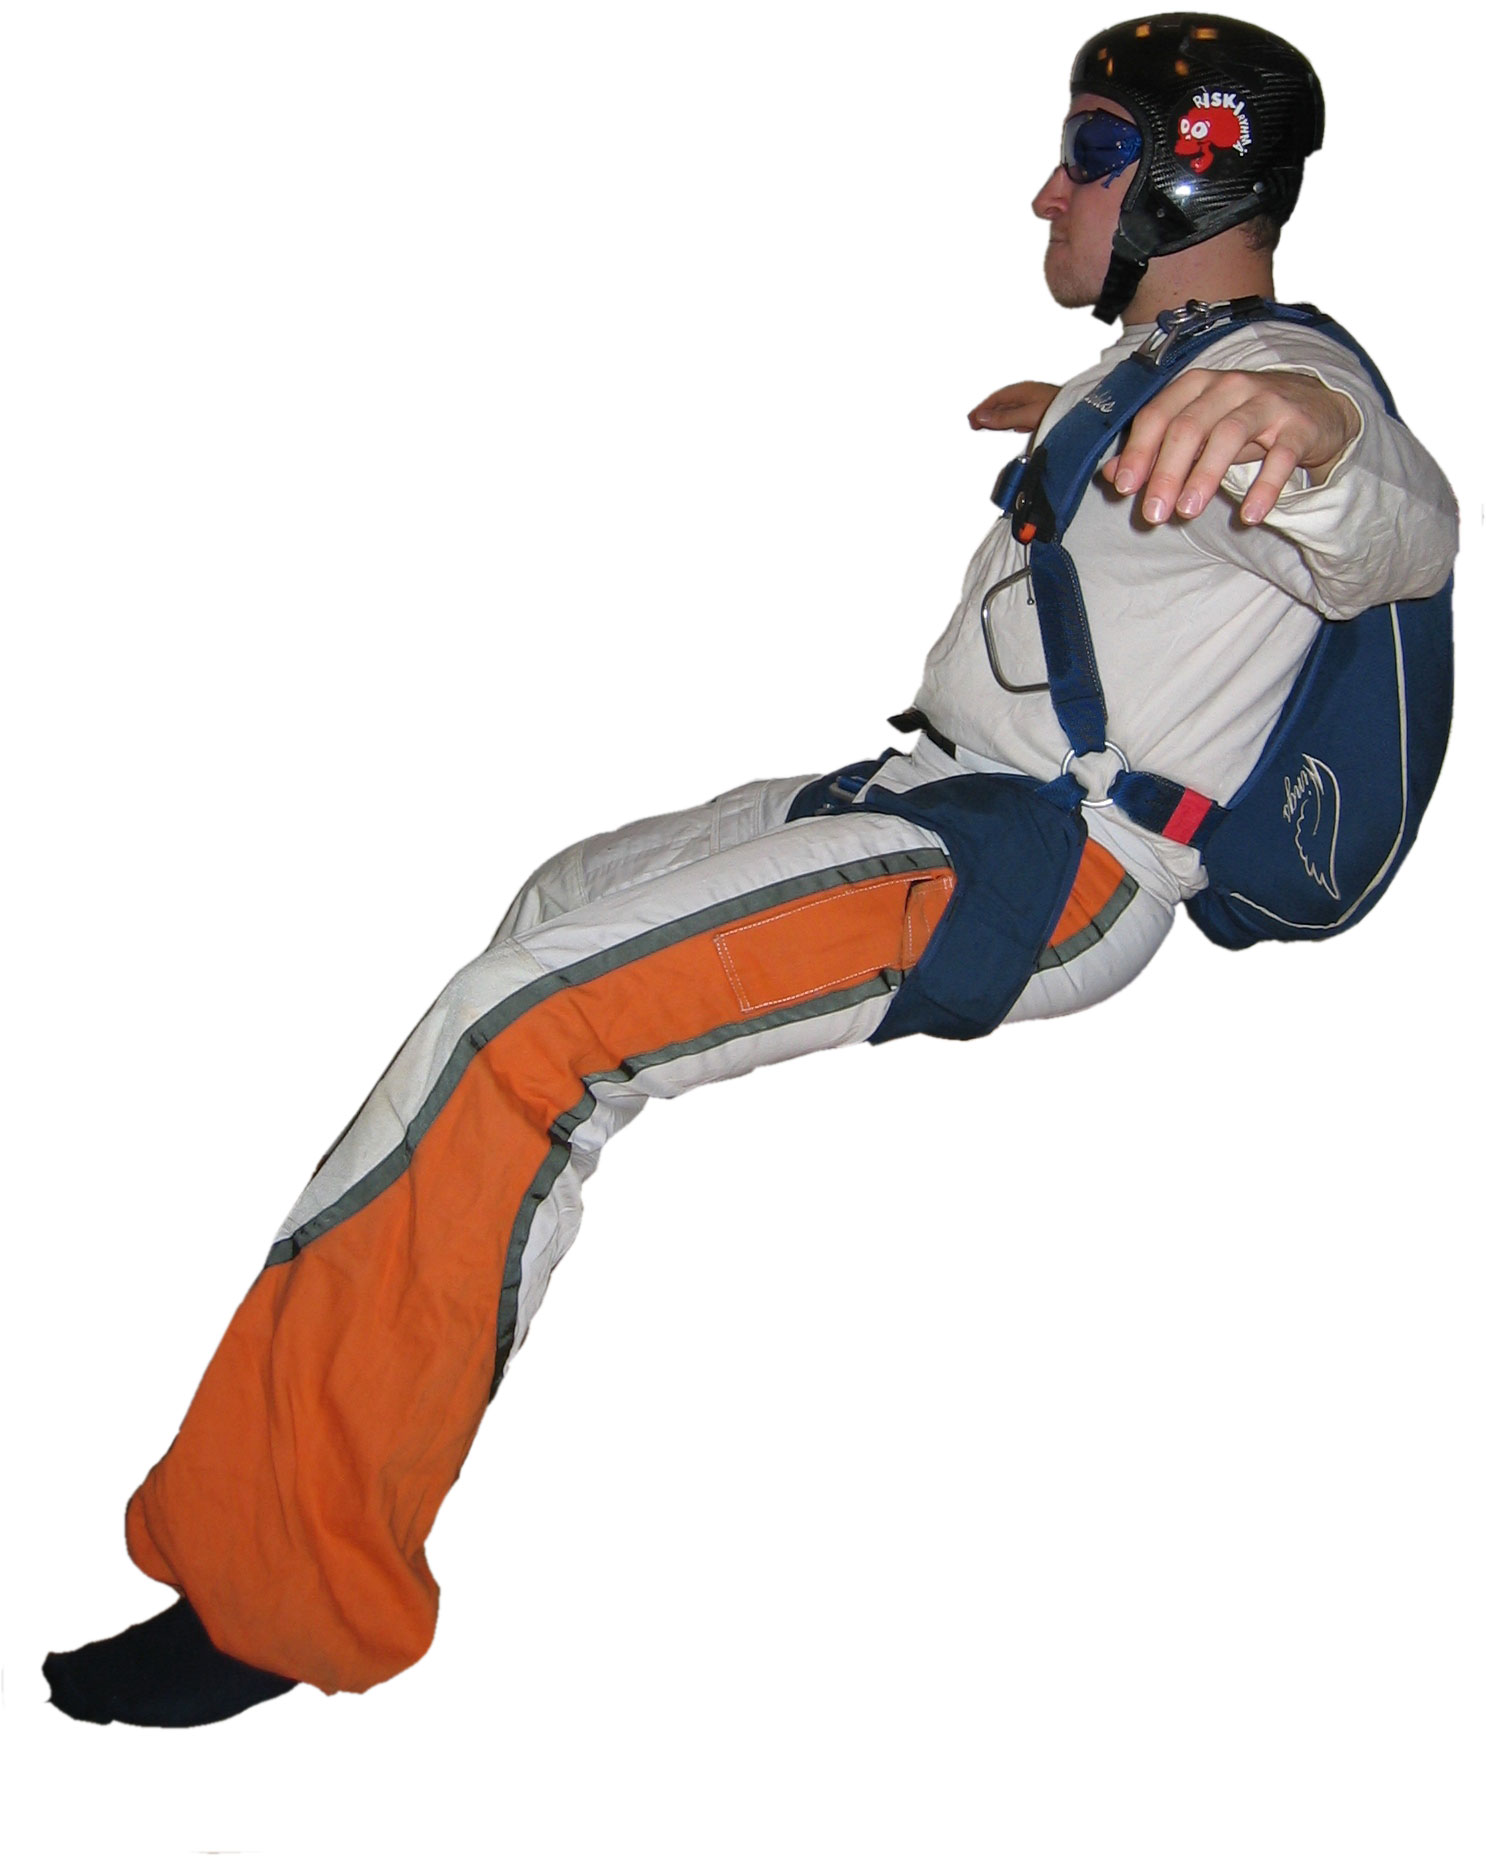
\includegraphics[width=0.7\textwidth]{Sittis-sivulta.jpeg}\captionof{figure}{Liikkuminen eteenpäin sittiksessä}\end{Figure} 


Painamalla lantiota taaksepäin ja ylävartaloa eteenpäin liikut taaksepäin. Taaksepäin liikkuessa korostuu jalkojen hartioita leveämpi haara-asento, koska silloin alhaalta tuleva ilmavirta osuu suoraan ylävartaloon tehostaen taaksepäin menevää liikettä. Mikäli reitesi ovat liian lähellä toisiaan, muodostuu jaloista ja rintakehästä sinua ylöspäin nostava kuppi, jolloin liikut sekä taaksepäin että ylöspäin. 

\begin{verbatim}                                
\end{verbatim}

\begin{Figure}\centering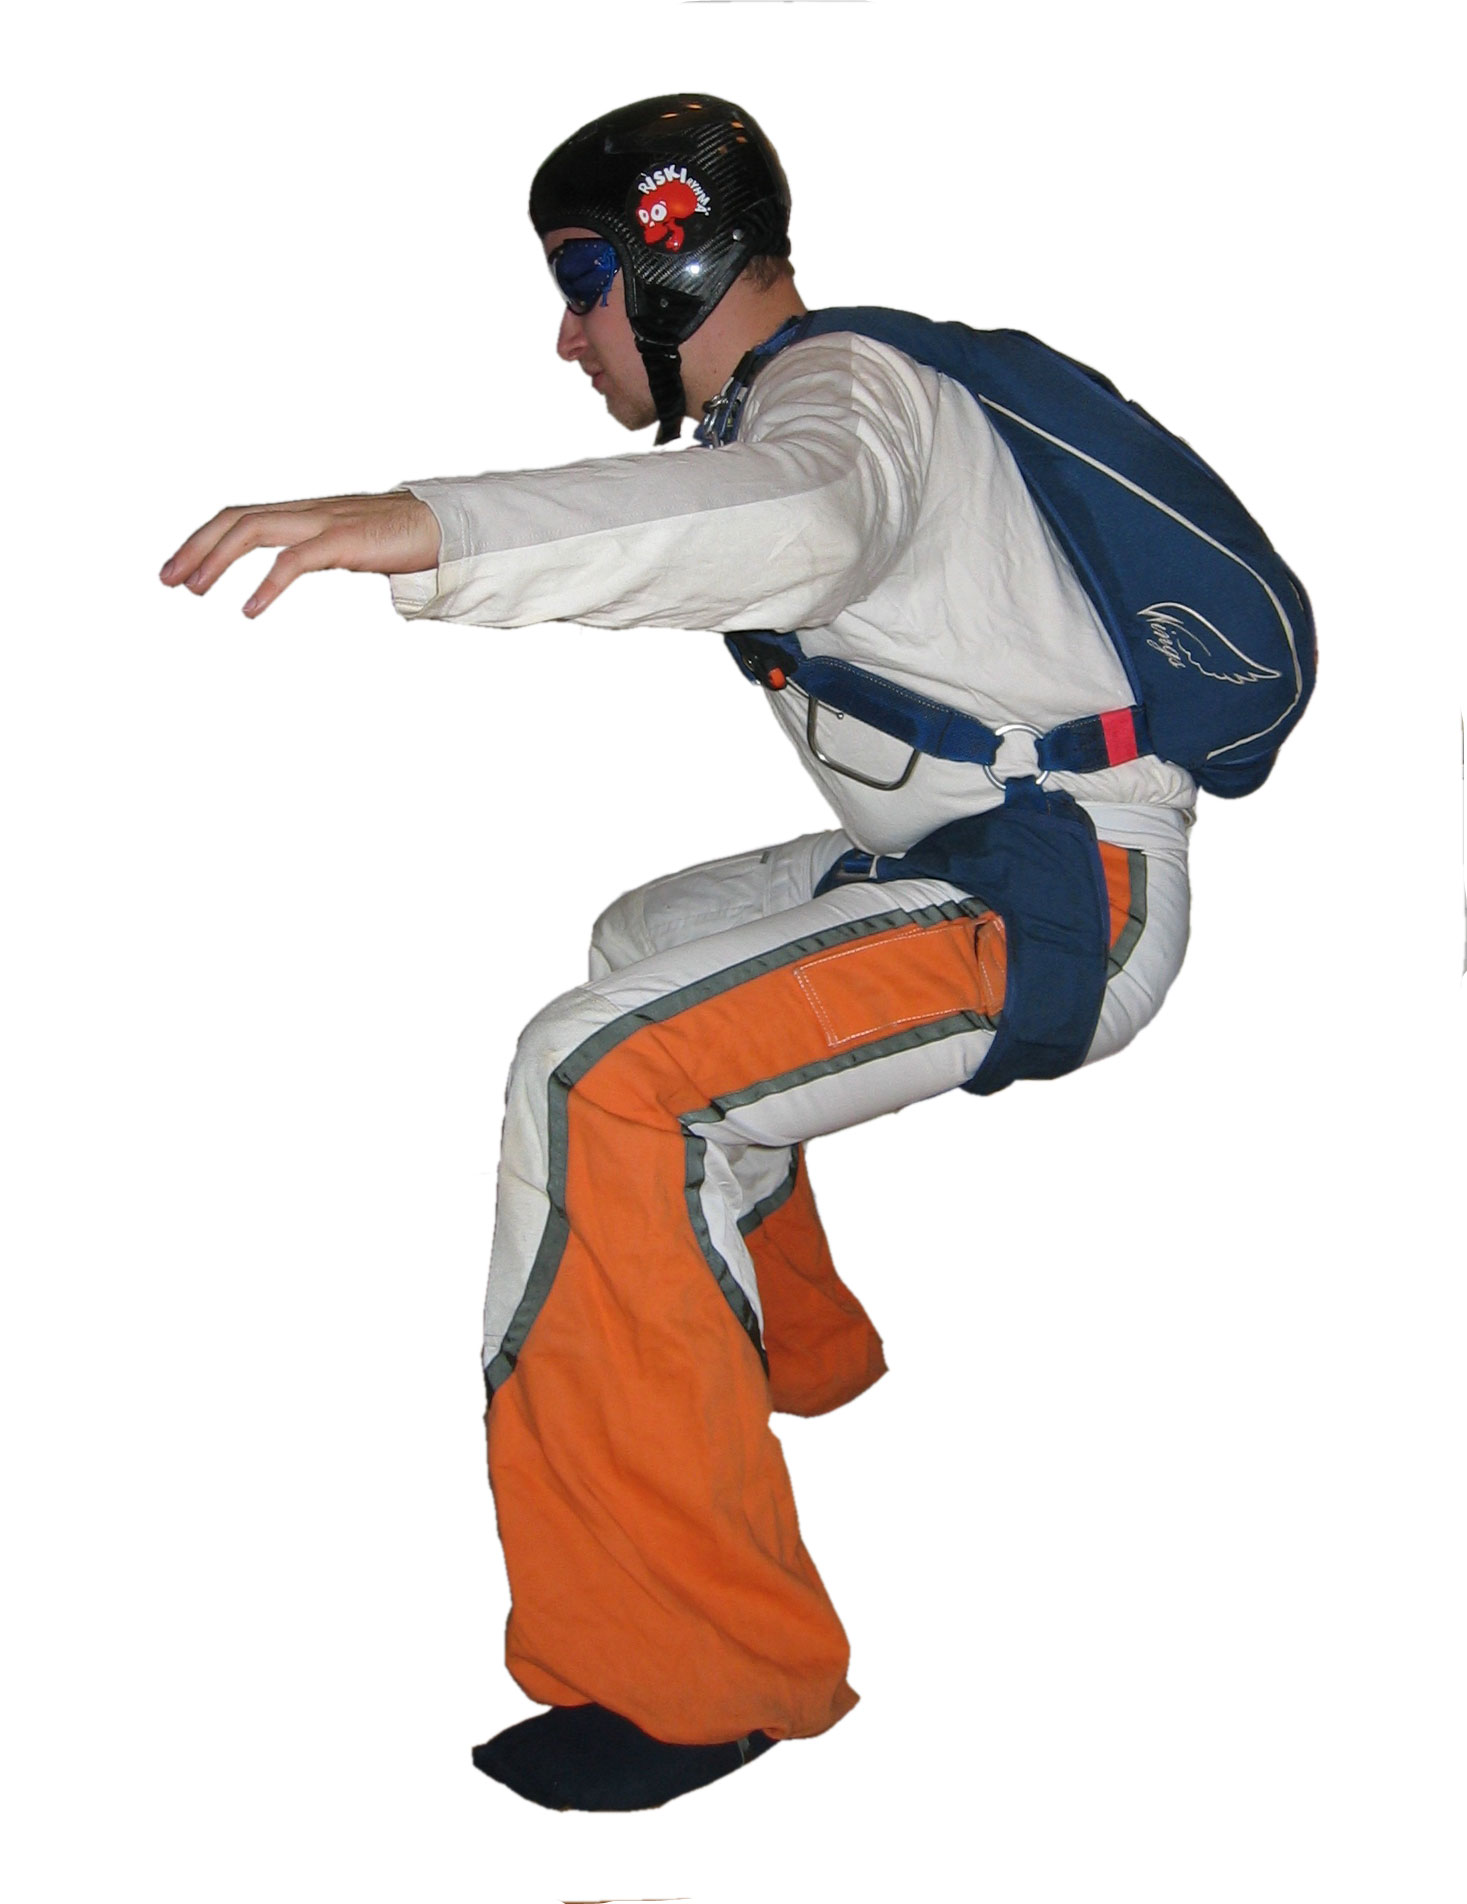
\includegraphics[width=0.7\textwidth]{Sittis-taaksepain.jpeg}\captionof{figure}{Liikkuminen taaksepäin sittiksessä}\end{Figure} 

\subsection{ Liikkuminen ylös- ja alaspäin sittiksessä }
\label{freefly-lentoasennot-liikkuminen-ylos-ja-alaspain-sittiksessa}


Liikkuaksesi alaspäin eli nopeammin, laske reisiäsi lantioon nähden alemmas tuoden polvia samalla lähemmäs toisiaan. Tarvittaessa vie jalat vartalon alle lähelle standup-asentoa. Sittiksessä voit lisätä vauhtia myös pelkästään nostamalla käsivarsia ylöspäin. Muista, että kapeampi asento on epävakaampi lentää. 


Liikkuaksesi ylöspäin eli hitaammin, paina käsiäsi symmetrisesti alaspäin vasten ilmavirtaa ja levitä jalkojasi. Voit suoristaa jalkoja sivuille polvesta alaspäin tai painaa polvia sisäänpäin vasten ilmavirtaa – samaan tyyliin kuin maalivahti torjuu jalkojensa välistä menevän jääkiekon. Voit hidastaa vauhtia myös selkästabiililla, jolloin vauhti hidastuu huomattavasti, mutta pidä huoli, ettet korkkaa ja osu muihin hyppääjiin. 

\subsection{ Mikä voi mennä vikaan sittiksessä? }
\label{freefly-lentoasennot-mika-voi-menna-vikaan-sittiksessa}


Jos päädyt selällesi, 

\begin{itemize}
\item  et ehkä pidä jalkojasi tarpeeksi voimakkaasti oikeassa asennossa polvesta alaspäin (ilmavirran ei pitäisi osua suoraan pohkeisiin eikä sääriin). 
\item  kätesi ovat ehkä liian edessä. 
\item  selkäsi ei ehkä ole suorassa. 
\end{itemize}

Jos päädyt mahallesi: 

\begin{itemize}
\item  Polvesi eivät ehkä ole 90 asteen kulmassa vaan kantapäät osoittavat takapuoleesi ja ilmavirta ottaa sääriisi. 
\item  Selkäsi ei ehkä ole suorassa. 
\end{itemize}

Jos pyörit holtittomasti: 

\begin{itemize}
\item  Jalkapohjasi eivät välttämättä osoita suoraan alaspäin polviesi alla. Jos käännät jalkapohjia osoittamaan edes hiukan sivulle alat pyörimään. 
\item  Käsivarret eivät ehkä ole symmetrisesti ilmaa vastaan, vaan toinen on ylempänä kuin toinen. 
\item  Jalkasi saattavat olla liian lähellä toisiaan. 
\end{itemize}

Jos joudut yllä mainitun kaltaiseen epästabiiliin tilaan, mene palloasentoon ja yritä uudelleen. 

\subsection{ Käännökset sittiksessä }
\label{freefly-lentoasennot-kaannokset-sittiksessa}


Sittiksestä voit tehdä käännöksen seuraavalla tavalla. Ota kiintopiste edestäsi. Paina käännöksen puoleista kättäsi hieman alaspäin ja hartialinjasi taakse. Katso käännöksen suuntaan pitäen katse horisontissa. Sittisasentosi lähtee kääntymään. Pidä katse koko käännöksen ajan horisontissa. Muista pitää jalkojen asento voimakkaasti sittiksen perusasennossa käännöksen aikana. Älä käännä sääriä reisien alle. Tee käännöksen pysäytys ajoissa ennen kiintopistettä suoristamalla ylävartalo sekä käsien vastaliikkeellä. Yleensä käännös onnistuu pelkästään ajatuksen voimalla. 


Käännöstä voi nopeuttaa muodostamalla käsistä ja jaloista potkurin lavat. Näin tehtäessä käännös on voimakas ja asento epävakaampi. Harjoittelun alkuvaiheessa opettele käännös pelkästään käsiä käyttämällä niin kuin yllä on kuvailtu. 

\section{ Pää alaspäin lentäminen  }
\label{freefly-lentoasennot-paa-alaspain-lentaminen}


Pää alaspäin (head down, hetukka) lentämisessä on monia tyylejä ja niiden risteytyksiä. Tärkeintä hetukan lentämisessä on se, että hallitset omalla tyylilläsi paikallaan lentämisen, liikkumisen eri suuntiin, osaat pysäyttää liikkeen sekä pystyt havainnoimaan ympäristösi muutokset vapaapudotuksen aikana. Sinun tulee hallita sittislentämisen perusteet ennen hetukan opettelua. Jos hetukkahyppy karkaa hallinnasta, sinun on pystyttävä stabiloimaan lentoasentosi nopeasti sittikseen, jotta et korkkaa ja siten aiheuta muille tai itsellesi vaaraa ja loukkaantumisia. 

\subsection{ Head down asennon harjoittelu }
\label{freefly-lentoasennot-head-down-asennon-harjoittelu}


Hetukan perusasento on straddle-asento. Suomeksi straddle tarkoittaa ”istua hajareisin” tai ”istua kuten hevosen selässä”. Edestäpäin straddle-asento näyttää putoavalta sulkapallolta. Tähän perusasentoon pääset joko sittiksestä tai suoraan uloshypystä. Sittiksestä pääset päällesi sivukautta (puolikas kärrynpyörä) tai etukautta (kuin nousisit seisomaan päällesi etuvoltin kautta). Kun olet päälläsi: 

\begin{itemize}
\item  Levitä jalat leveään haaraan sivuille ja koukista niitä hieman polvista. Pidä pohkeet ilmavirrassa. Pyri siihen ettei kumpikaan jalkasi pääse retkahtamaan liikaa eteen tai taakse haukaten ilmaa. 
\item  Levitä käsivartesi sivuille, mutta pidä ne tarpeeksi matalalla, jottei niska ja hartiat jännity. Kämmenet taivasta kohti, kädet rentona. 
\item  Katso horisonttiin – muutaman hypyn jälkeen horisontin katsominen väärinpäin tuntuu jo luontevalta. 
\item  Pidä lantio ja niska selkärankaan nähden suorana. Koko ylävartalosi lantiosta päälakeen tulisi olla aivan suora. Yritä muutoin olla mahdollisimman rento. 
\item  Älä taivuta! 
\item  Muista hengittää! Jos sinusta tuntuu, että mikään ei onnistu, vedä syvään henkeä, rentoudu ja yritä uudelleen. 
\end{itemize}

\begin{Figure}\centering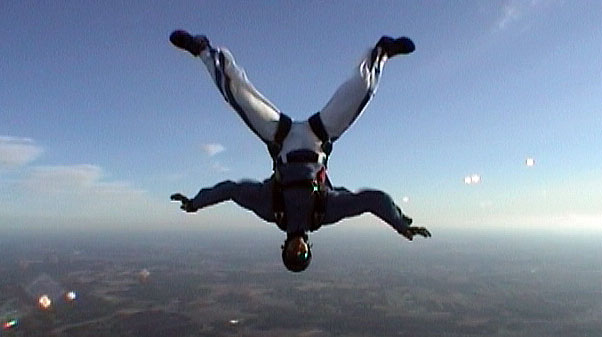
\includegraphics[width=0.95\textwidth]{Headdown-straddle.jpeg}\captionof{figure}{Straddle-asento}\end{Figure} 


Hetukka-asentoon pääseminen suoraan uloshypystä on helpointa, jos kiipeät ovella ulos niin, että selkäsi tai rintakehäsi on valmiiksi kohtisuoraan ilmavirtaan. Pudottaudu irti koneesta pystysuoraan straddle-asentoon ja anna ilmavirran kääntää sinut päällesi. Älä ponnista äläkä hyppää selälleen/mahalleen! Älä myöskään etsi horisonttia väkisin. Jos onnistut pudottautumaan ilmavirtaan oikein, asentosi kääntyy päälleen automaattisesti ja horisontti tulee näköpiiriisi. Usein on helpompaa opetella uloshyppyä niin, että pitää kädet ristissä rinnan päällä, jolloin sulkapallomainen asento kääntyy helpommin päälleen. Kädet avataan symmetrisesti lentoasentoon vasta kun horisontti on kääntynyt näköpiiriin. 


Harjoittelun alkuvaiheessa asento on usein liian jäykkä. Toinen yleinen ongelma on se, että hartioissa on taivutusta ja käsillä lennetään liikaa. Tavoitteena on lentää enimmäkseen jaloilla ja lantiolla, jolloin kädet vapautuvat esimerkiksi otteiden ottamiseen, asennon stabiloimiseen ja vauhdin säätelemiseen. 


Opetellessasi hetukkaa, pidä asentoa vain viitisen sekuntia kerrallaan. Vaihda takaisin sittikseen, käänny poikki hyppylinjan ja käänny uudelleen päällesi. Näin vauhtisi pysyy kohtuullisena ja voit kontrolloida tahatonta liikkumista. Kun harjoittelet hetukka-asentoa, tee se aina poikkilinjaan! 

\subsection{ Daffy }
\label{freefly-lentoasennot-daffy}


Lennettäessä pää alaspäin daffy-asento on hyvin monikäyttöinen lentoasento. Daffyssa voit helposti säädellä nopeutta ja paikkaa sekä lentää otetta. Daffyssa ylävartalo on kuten straddlessa – vain jalkojen asento on erilainen. Daffyssa toinen jalka tuodaan suoraan vartalon etupuolelle. Jalka on lantiosta ja polvesta taivutettuna ja ilmavirran tulee tuntua etureidessä ja säären edessä. Toinen jalka viedään suoraan taakse ja sitä taivutetaan polvesta. Ilmavirran tulee tuntua sen jalan takareidessä ja pohkeessa. Takajalan on oltava hivenen enemmän ilmavirrassa kuin etujalan, jotta asento pysyy paikoillaan. Jalkojen tulee olla rennot ja ylävartalon ilmavirtaan nähden suora tai muutoin asento saattaa lähteä pyörimään. 


Lennettäessä pää alaspäin Daffy on hyvin monikäyttöinen lentoasento. Daffyssä voit helposti säädellä nopeutta, paikkaa ja sekä lentää otetta. Pidä katse horisontissa, muista hengittää ja olla rento. 


\begin{Figure}\centering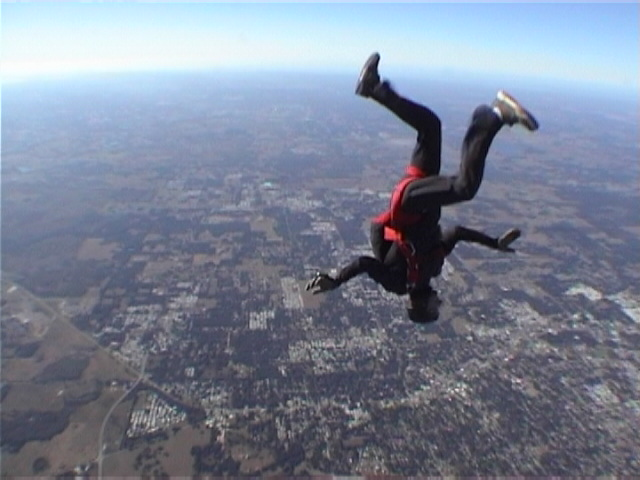
\includegraphics[width=0.95\textwidth]{Daffy.jpeg}\captionof{figure}{Daffy}\end{Figure} 

\subsection{ Shelf }
\label{freefly-lentoasennot-shelf}


Shelf-asento on alunperin tuulitunnelissa kehitetty. Siinä jalat vievät mahdollisimman vähän tilaa. Molemmat jalat ovat lantiosta hieman taivutettuna, polvista taakse taivutettuna, niin että asento ikään kuin roikkuu takana olevien säärien varassa. 


Oppiessasi enemmän head downia, opit muuttamaan jalkojesi asentoa straddlen ja daffyn ja shelfin välillä tilanteesta riippuen. Ei siis ole yhtä ainoaa oikeaa asentoa. Kuitenkin head downia opetellessa kannattaa ensin opetella yksi jalkojen asento ja liikkuminen siinä ja sen jälkeen lähteä opettelemaan jalkojen asennon muuttamista. 

\subsection{ Liikkuminen eteen- ja taaksepäin }
\label{freefly-lentoasennot-liikkuminen-eteen-ja-taaksepain}


Horisontaalinen liikkuminen vapaapudotuksessa on periaatteeltaan aina samanlainen riippumatta lentoasennosta. Jos haluat liikkua tiettyyn suuntaan, on ilmavirrassa olevan pinta-alan vastakkaisella puolella oltava suurempi. Sinun tulee miettiä, mistä ilmavirta tulee ja mihin suuntaan se sinua työntää liikuttaessasi käsiäsi, jalkojasi ja vartaloasi eri asentoihin. Head downissa erittäinkin pienet liikkeet ja muutokset vartalon asennossa aiheuttavat jo liikkeen vastakkaiseen suuntana. 


Liikkuminen hetukan perusasennossa (straddle) tapahtuu lantiota ja jalkoja käyttäen. Liikkuaksesi eteenpäin paina lantiota taaksepäin, jolloin lantio ja alaselkä osuvat ilmavirtaan ja se vie sinua eteenpäin. Eteenpäin menevää liikettä voit tehostaa painamalla jalkoja korostetusti ilmavirtaa vasten. Ilmavirta tuntuu tällöin takareisissä ja pohkeissa. Taaksepäin liikkuaksesi paina lantiota eteenpäin, jolloin ilmavirta osuu alavatsaan ja lantioon. Taaksepäin menevää liikettä voit tehostaa painamalla etureidet ilmavirtaan. 


Horisontaalinen liikkuminen daffy-asennossa tapahtuu jalkoja ja lantiota käyttämällä. Eteenpäin liikutaan painamalla takimmaista jalkaa ilmavirtaa vasten ja siirtämällä etummaista jalkaa pois ilmavirrasta. Eteenpäin pääsy tehostuu viemällä lantiota taakse. Taaksepäin liikkuminen tapahtuu päinvastoin. 


Kun liikut eteen tai taakse, vartalosi pinta-ala ilmavirtaan nähden on suurempi kuin suoraan alaspäin putoavassa lentoasennossa. Tämä aiheuttaa sinulle hitaamman putoamisnopeuden verrattuna suoraan alaspäin putoaviin hyppääjiin. Jotta putoat yhtä nopeasti kuin he, joudut kaventamaan joko jalkojesi tai käsiesi asentoa (eli pienentämään ilmavirrassa olevaa pinta-alaa). 

\subsection{ Liikkuminen ylös- ja alaspäin }
\label{freefly-lentoasennot-liikkuminen-ylos-ja-alaspain}


Vertikaalista liikkumista tarvitset esimerkiksi päästäksesi hyppykaverisi kanssa samalle tasolle. Putoamista nopeutetaan kaventamalla perusasentoa. Käsiin ja jalkoihin osuvaa pinta-alaa täytyy siis pienentää vauhdin kiihdyttämiseksi. Muista pitää katse hyppykaverissasi, ettet ajaudu hänen päälleen tai törmää häneen! Pysäyttäminen tapahtuu levittämällä lentoasento takaisin normaaliksi. Huomioi, että sinun on aloitettava hidastaminen huomattavasti aikaisemmin kuin esimerkiksi mahallaan lentäessä. Mikäli et aloita jarruttamista ajoissa, putoat hyppykaverisi alapuolelle. 


Putoamisvauhtia hidastetaan lisäämällä hetukka-asennon pinta-alaa levittämällä jalkoja ja käsiä. Käsien levittämisen haittana on se, että kädet ottavat vastaan enemmän ilmavirtaa kuin normaalisti, jolloin et voi käyttää niitä rennosti esimerkiksi otteisiin. Helpompi ja tehokkaampi tapa hidastaa vauhtia on daffy-lentoasennon käyttäminen, jolloin jalat ottavat vastaan huomattavasti enemmän ilmavirtaa ja hidastavat näin putoamisvauhtia. Daffyssa kädet jäävät vielä rennoksi otteita varten, mutta niitä voi myös levittää hidastumisen tehostamiseksi. 


\begin{Figure}\centering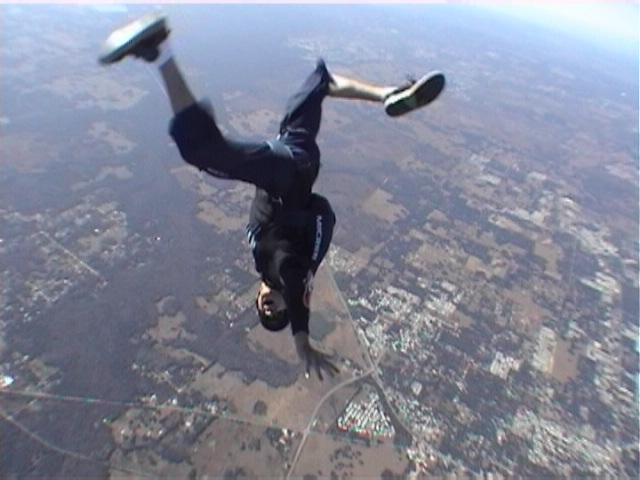
\includegraphics[width=0.95\textwidth]{Daffy-sivulta.jpeg}\end{Figure} 


Kun pyrit pitämään pään samalla tasolla muiden hyppääjien kanssa, alat vähitellen oppia luontaisesti korjaamaan putoamisnopeuttasi verrattuna muihin hyppääjiin sitä juurikaan miettimättä. 

\subsection{ Käännökset head downissa }
\label{freefly-lentoasennot-kaannokset-head-downissa}


360 asteen käännöksen voi tehdä hetukassa esimerkiksi hartioilla tai jaloilla. Hartioilla tehty käännös aiheuttaa ilmassa ovaalin muotoisen kierroksen. Jaloilla oikein tehty käännös pyörähtää paikoillaan. Hartioita apuna käyttäen käännös tehdään seuraavasti. Ota kiintopiste horisontista tai kanssahyppääjästä. Katso aikomasi käännöksen suuntaan, jolloin hartiat kääntyvät automaattisesti pään käännön mukana ja alat kääntyä katseesi mukaiseen suuntaan. Pidä katse horisontissa, jotta asento pysyy vakaana. Pysäytä käännös kiintopisteen tai kanssahyppääjän kohdalla ottamalla normaali rento lentoasento. 


Myös jalkakäännöksessä tarvitset kiintopisteen horisontista tai kanssahyppääjästä. Tee kääntymissuunnan puoleisella jalalla pieni liike eteenpäin ja kääntymissuunnan vastakkaisella jalalla pieni liike taaksepäin. Tämä jalkojen liike ohjaa ilmavirran kääntämään sinua. Mitä suurempi liike jaloilla tehdään, sitä nopeammin asento kääntyy. Pidä katse horisontissa koko käännöksen ajan, jotta lentoasento pysyy vakaana. Pysäyttääksesi kääntymisen, tee molemmilla jaloilla yhtäaikainen vastaliike hyvissä ajoin ennen horisontista otettua kiintopistettä tai kanssahyppääjää, koska jalkakäännös kääntyy nopeammin kuin hartioilla tehty käännös. Ota lopuksi kiintopisteen tai kanssahyppääjän kohdalla normaali rento lentoasento. 


\begin{figure*}[]\centering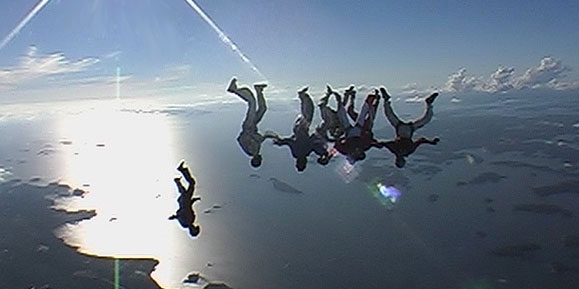
\includegraphics[width=0.95\textwidth]{Headdown-ryhma.jpeg}\end{figure*} 

\subsection{ Otteet }
\label{freefly-lentoasennot-otteet}


Otteiden ottaminen hetukassa ei ole aina itsetarkoitus. Tärkeämpää ja jopa vaikeampaakin on pystyä lentämään omaa paikkaa. Otteen ottaminen ei saa vaikuttaa lentämiseen eikä lentämistä pidä koskaan lopettaa kun ote on saatu. 


Kun lähdet ottamaan otetta, sinun on oltava samalla tasolla hyppykaverin kanssa. Tämän jälkeen lennetään horisontaalinen etäisyys kiinni ja pysäytetään liike. Ennen otteen ottamista on hyvä lentää hetki paikallaan ote-etäisyydellä ottamatta toisesta kiinni. Otetta otettaessa on tärkeää keskittyä omaan lentämiseen – kurottaminen ei kannata ja hyppykaverissa ei saa roikkua. 


Otteessa olevan käden käsivarren tulee olla hieman koukussa siten, että ote on joustava pienelle liikkeelle. Käsivarren pitää pysyä hartialinjan alapuolella. Jos otetta kurotetaan, siitä tulee jäykkä ja siihen tulee vetoa. Irrota ote heti, jos se ei tunnu hyvältä. Ote, jossa on vetoa, vaikeuttaa muidenkin lentämistä paikoillaan. Ote on hyvä, kun pystyt pitämään hyppykaverista kiinni rennosti ja kevyesti. 

